%\documentclass[showpacs,preprintnumbers,amsmath,amssymb,superscriptaddress,aip]{revtex4-1}
\documentclass[twocolumn,showkeys,superscriptaddress]{revtex4}
\usepackage{graphicx}
%\usepackage{authblk}
%\usepackage{amssymb}
%\setlength{\parindent}{0in}

% General Latex  --------------------------------------------------
\def\beq{\begin{equation}}
\def\eeq{\end{equation}}
\def\beqar{\begin{eqnarray}}
\def\eeqar{\end{eqnarray}}
\def\nn{\nonumber}
\def\ol{\overline}
\def\para{\parallel}

% Operators  ------------------------------------------------------
\newcommand{\diff}[2]{\frac{d#1}{d#2}}
\newcommand{\diffs}[2]{\frac{d^2#1}{d#2^2}}
\newcommand{\pdiff}[2]{\frac{\partial#1}{\partial#2}}
\newcommand{\pdiffs}[2]{\frac{\partial^2#1}{\partial#2^2}}
\newcommand{\pdiffxy}[3]{\frac{\partial^2#1}{\partial#2 \partial#3}}
\newcommand{\pdt}{\partial_t}
\newcommand{\pdr}{\partial_r}
\newcommand{\pdth}{\partial_\theta}
\newcommand{\pdrr}{\partial^2_r}

\newcommand{\enum}[2]{{#1}\times10^{#2}} % 4.2x10^{3} = \enum{4.2}{3}

\newcommand{\vect}[1]{{\bf #1}}
%\newcommand{\vect}{\overrightarrow}
%\newcommand{\vect}{\vec}
\def\div{\nabla\cdot}
\def\grad{\nabla}
\def\curl{\nabla\times}
\newcommand{\gradpar}{\grad_\parallel}
\newcommand{\gradperp}{\grad_\perp}
\newcommand{\gradr}{\grad_r}
\newcommand{\defeq}{\ensuremath{\stackrel{\text{\tiny def}}{=}}}

\newcommand{\savg}[1]{\left<{#1}\right>}
\newcommand{\vavg}[1]{\left<{#1}\right>_V}
\newcommand{\thavg}[1]{\left<{#1}\right>_\theta}

% Variable names  -------------------------------------------------
\newcommand{\vpar} {v_\parallel}
\newcommand{\Apar} {A_\parallel}
\newcommand{\jpar} {j_\parallel}
\newcommand{\kpar} {k_\parallel}
\newcommand{\kperp} {k_\perp }
\newcommand{\vperp} {v_\perp }
\newcommand{\kthe}{k_\theta}

\newcommand{\Evec}{\ensuremath{\boldsymbol{{\rm E}}}}
\newcommand{\Bvec}{\ensuremath{\boldsymbol{{\rm B}}}}
\newcommand{\Jvec}{\ensuremath{\boldsymbol{{\rm J}}}}
\newcommand{\Fvec}{\ensuremath{\boldsymbol{{\rm F}}}}
\newcommand{\fvec}{\ensuremath{\boldsymbol{{\rm f}}}}
\newcommand{\vE}{\ensuremath{\boldsymbol{{\rm v}_{E}}}}
\newcommand{\bo}{\ensuremath{\boldsymbol{{\rm b}_0}}}
\newcommand{\bvec}{\ensuremath{\boldsymbol{{\rm b}}}}
\newcommand{\xvec}{\ensuremath{\boldsymbol{{\rm x}}}}
\newcommand{\yvec}{\ensuremath{\boldsymbol{{\rm y}}}}
\newcommand{\zvec}{\ensuremath{\boldsymbol{{\rm z}}}}
\newcommand{\vvec}{\ensuremath{\boldsymbol{{\rm v}}}}
\newcommand{\jvec}{\ensuremath{\boldsymbol{{\rm j}}}}

\newcommand{\bxgp}{\bvec\times\gradperp}

\newcommand{\vve}{\ensuremath{\boldsymbol{{\rm v}}_{e}}}
\newcommand{\vvi}{\ensuremath{\boldsymbol{{\rm v}}_{i}}}
\newcommand{\vpe}{v_{\parallel e}}
\newcommand{\vpi}{v_{\parallel i}}
\newcommand{\vvE}{\ensuremath{\boldsymbol{{\rm v}}_{E}}}
\newcommand{\vvD}{\ensuremath{\boldsymbol{{\rm v}}_{D}}}

\newcommand{\nuei}{\nu_{ei}}
\newcommand{\nuii}{\nu_{ii}}
\newcommand{\nue}{\nu_{e}}
\newcommand{\nuen}{\nu_{en}}
\newcommand{\nuin}{\nu_{in}}
\newcommand{\kpe}{\kappa_{\parallel e}}

\newcommand{\rs}{\rho_{s}}
\newcommand{\ri}{\rho_{i}}
\newcommand{\wci}{\Omega_{i}}
\newcommand{\wcix}{\Omega_{ix}}
\newcommand{\wce}{\Omega_{e}}
\newcommand{\tomega}{\tilde\omega}
\newcommand{\Isat}{I_{\rm sat}}
\newcommand{\fmie}{\frac{m_i}{m_e}}
\newcommand{\fmei}{\frac{m_e}{m_i}}


% Often used dimensions
\newcommand{\cm}{\rm cm}
\newcommand{\mm}{\rm mm}
\newcommand{\cmn}{{\rm cm}^{-3}}
\newcommand{\mn}{{\rm m}^{-3}}
\newcommand{\eV}{\rm eV}
\newcommand{\G}{\rm G}
\newcommand{\T}{\rm T}



\begin{document}

\title{A Procedure to Predict the Subcritical Turbulent Onset Criterion Applied to a Modified Hasegawa-Wakatani Model}

\author{B. Friedman}
\email{friedman@physics.ucla.edu}

\affiliation{Department of Physics and Astronomy, University of California, Los Angeles, California 90095-1547, USA}
\affiliation{Lawrence Livermore National Laboratory, Livermore, California 94550, USA}


\author{T.A. Carter}

\affiliation{Department of Physics and Astronomy, University of California, Los Angeles, California 90095-1547, USA}



\begin{abstract}

\end{abstract}

\maketitle

\section{Introduction}

Turbulence in magnetically confined plasmas is almost always attributed to linear instabilities. The calculation of linear instabilities through normal mode analysis
-- the calculation of eigenvalues and eigenvectors of a linearized dynamical system -- has successfully predicted the onset criterion for many MHD and micro-instabilities.
Nevertheless, it is well-known in the hydrodynamics community that normal mode analysis fails at predicting turbulent onset for a large class of experiments, in which the
turbulence is called subcritical~\cite{drazin1981}. 
In these experiments, turbulence appears even though all linear eigenvectors are stable, meaning infinitesimal perturbations on the laminar state cannot grow exponentially. 
Nevertheless, finite amplitude perturbations can still excite turbulence.
Subcritical turbulence is certainly possible in plasmas as well, and several instances have been studied in the 
past~\cite{waltz1985,scott1990,nordman1993,biskamp1995,drake1995,itoh1996,camargo1998,krommes1999,camporeale2009,schekochihin2012,highcock2012}. 
For the most part, however, normal mode analysis dominates plasma turbulence prediction despite the fact that it is not useful in all instances.

Since the hydrodynamics community has long studied subcritical turbulence, it has much to offer in terms of understanding of the phenomenon. Most significantly,
in the early 1990s, several researchers attributed the failure of normal mode analysis in predicting subcritical turbulent onset to the non-normality of linear operators of
dynamical systems~\cite{gustavsson1991,butler1992,trefethen1993,reddy1993,henningson1994,schmid2007}. A non-normal operator has 
eigenvectors that are not orthogonal to one another. One consequence of eigenvector nonorthogonality is that even when all eigenvectors decay exponentially under linear evolution, 
superpositions of eigenvectors can grow, albeit transiently.
In other words, certain fluctuations of the laminar state can access free energy from background gradients even though normal mode fluctuations cannot.
When combined with nonlinear effects, this allows for sustained subcritical turbulence by a bootstrapping process.
Such behavior is obscured by traditional normal mode analysis, which only effectively describes the long time asymptotic behavior of fluctuations under  
action of the linear operator. Transient growth, which can dominate turbulent evolution, can be discovered only through non-modal calculations.

Non-modal analysis generally employs tools such as pseudospectra and maximum growth curves, which have been used to successfully explain why turbulence is subcritical in various instances. 
However, they have not been used to predict onset criteria in subcritical systems (e.g. the transition Reynold's number in pipe flows).
This paper outlines and illustrates a non-modal linear method to make quantitative predictions of turbulent properties including turbulent onset criteria. 
Our approach is to define a non-modal growth rate that is analagous to an eigenmode growth rate, but which takes into account transient growth effects. To accomplish this, we make
several simplifying assumptions regarding the nonlinearities; namely, the nonlinearities randomize the spatial structures of the turbulence on a characteristic nonlinear time scale, which can
be estimated by a characteristic linear time scale.

More specifically, we model the turbulent steady state as a series of processes:  (1) the turbulence starts as a spatially random state, 
(2) linear transient growth deterministically amplifies the turbulent energy (or depresses it, depending on the wavenumber), 
(3) nonlinear transfer sets in at a specified timescale, terminating the transient growth process and re-randomizing the turbulent state (at which point the cycle repeats). 
Optimally, the timescale for the final step would be the nonlinear decorrelation time of the turbulent system, but in order to enable predictive capability, we employ critical balance
arguments to use a characteristic linear time. The procedure ultimately produces a growth rate that can be used to predict turbulent properties such as saturation levels and transport rates 
through mixing length arguments. Furthermore, a finite positive growth rate (of a certain magnitude) indicates that turbulence can exist given a sufficient amount of noise in the system.
Thus, the growth rate provides a turbulent onset criterion, even for subcritical systems.

The paper is organized as follows: in Section~\ref{sec_hw_model}, we specify our illustrative model -- the 2D and 3D Hasegawa-Wakatani model -- 
that we use throughout the paper and describe its linear non-normal properties,  while in Section~\ref{sec_non_norm_turb}, we explore the effect of linear non-normality in the model on turbulence. 
In Section~\ref{sec_nm_procedure}, we cover the details of our non-modal predictive procedure and show its success in predicting properties of highly non-normal turbulence. 
Finally, in Section~\ref{sec_subcrit_prediction}, we modify the 3D Hasegawa-Wakatani model to make it subcritical and show how our non-modal technique predicts the critical gradient for the onset of turbulence.

\section{Non-Normality of the Hasegawa-Wakatani Model} 
\label{sec_hw_model}

In order to illustrate and test our non-modal technique, we use as an example the well-known and well-analyzed Hasegawa-Wakatani (HW) model~\cite{hasegawa1983}.
In this section, we analyze the linear normality of the model.
We consider both the original 2D and the extended 3D~\cite{biskamp1995} versions of the model in a straight, unsheared magnetic field. 
The HW model consists of two equations for the density $n$ and the electrostatic potential $\phi$. The 3D version of the model is

\beqar
\label{n_eq}
\pdiff{n}{t} = - {\mathbf v_E} \cdot \grad n - \kappa \pdiff{\phi}{y} + \xi \gradpar^2 (n - \phi) - D \gradperp^4 n, \\
\label{phi_eq}
\pdiff{\gradperp^2 \phi}{t} = - {\mathbf v_E} \cdot \grad (\gradperp^2 \phi) + \xi \gradpar^2 (n - \phi) - D \gradperp^6 \phi
\eeqar
The normalizations are $\phi \to e \phi/T_e, n \to n/n_0, \grad \to \rho_s \grad , x,y,z \to x,y,z/\rho_s, t \to \omega_{ci} t $. Additionally,
$\mathbf{v_E} = \mathbf{b} \times \grad \phi$, $\xi = 4 \pi \omega_{ce}/\nu_{ei}$, 
and $\kappa = \rho_s/L_n$, where $L_n$ is the density scale length. The terms $D \gradperp^4 n$ and $D \gradperp^6 \phi$ are artificial hyper-diffusion and hyper-viscosity used to dissipate
energy on small scales. We set $D \to 10^{-5}$ except in Sec.~\ref{sec_subcrit_prediction} where we set it to $0.5$.
We associate the direction along $\mathbf{B}$ as the parallel or $z$ direction. The direction perpendicular $\mathbf{B}$ that
points opposite the density gradient is defined as the $x$ direction, and the $y$ direction is taken perpendicular to both of these.

In the analysis and numerical simulations, which we perform with the BOUT++ code~\cite{dudson2009}, we use periodic boundary conditions in
the $y$ and $z$ directions with zero-value boundaries in the $x$ direction. We use a domain size of $64 \rho_s \times 64 \rho_s \times 300 \rho_s$.
For the 2D version of the model, we replace $-\xi \gradpar^2$ with a single parameter $\alpha$ (definied as $\alpha = 4 \pi k_z^2 \rho_s^2 \omega_{ce} /\nu_{ei})$, 
which is commonly known as the adiabaticity parameter~\cite{camargo1995,camargo1998}. Additionally we use a domain size of $50 \rho_s \times 50 \rho_s$.
In numerical simulations, the turbulence can laminarize due to the build-up of $k_y=0$ density and potential structures~\cite{biskamp1995}. To prevent this, we subtract out the $k_y=0$
$n$ and $\phi$ components, which is the equivalent of adding source terms to Eqs.~\ref{n_eq} and~\ref{phi_eq}~\cite{friedman2012b}.

The degree of non-normality of the linear operator in the HW model is largely a function of the adiabaticity parameter~\cite{camargo1998}, or in the 3D case, of $\xi \gradpar^2$. 
Note that a matrix is normal if it commutes with its adjoint: $\mathbf{D} \mathbf{D}^\dagger = \mathbf{D}^\dagger \mathbf{D}$ for $\mathbf{D}$ normal. 
The HW model has a normal linear operator in the limit of $\alpha, \xi \gradpar^2 \to \infty$. 
To see this, we first transform the linear operator into a linear matrix by using a Fourier decomposition. Because we use a zero-value boundary condition in the $x$ direction, the
Fourier decomposition takes the form:

\beq
\label{fourier_form}
f_k = \int_0^{L_x,L_y,L_z} f(\mathbf{r}) \ {\rm sin} \left( k_x x \right) e^{i k_y y + i k_z z} d\mathbf{r}
\eeq
where $k_x = \pi l/L_x, k_y = 2 \pi m/L_y, {\rm and } \ k_z = 2 \pi n/L_z$ with $l, m, {\rm and } \ n$ integers.
The result for the 3D model is an equation for each mode $k = (k_x,k_y,k_z)$:

\beqar
\label{fourier_eqn}
\frac{\partial}{\partial t} \left( \begin{array}{cc} n_k \\ \phi_k \end{array} \right) = \mathbf{A}_k \left( \begin{array}{cc} n_k \\ \phi_k \end{array} \right) + \mathbf{N}_k \left( \begin{array}{cc} n_k \\ \phi_k \end{array} \right), \\ \nonumber \\
\label{A_k}
\mathbf{A}_k = \left( \begin{array}{cc} -\xi k_z^2 - D k_\perp^4 & -i \kappa k_y + \xi k_z^2 \\  \xi \frac{k_z^2}{k_\perp^2} & - \xi \frac{k_z^2}{k_\perp^2} - D k_\perp^4\end{array} \right)
\eeqar
with $\mathbf{A}_k$ being the linear coupling matrix and $\mathbf{N}_k$ the nonlinear matrix, which we don't write explicitly. 
Now in assessing the degree of normality of the HW model, we are not interested in the normality of $\mathbf{A}_k$ itself. 
Rather, we are interested in the energetically-weighted version of this matrix~\cite{camargo1998,schmid2007,camporeale2010}. Since the energy in a given Fourier mode is

\beq
\label{en_def}
E_k =  \frac{1}{2} \left( |n_k|^2 + k_\perp^2 |\phi_k|^2 \right).
\eeq
we rewrite Eq.~\ref{fourier_eqn} as

\beqar
\label{fourier_en_eqn}
\frac{\partial}{\partial t} \left( \begin{array}{cc} n_k \\ k_\perp \phi_k \end{array} \right) = \mathbf{B}_k \left( \begin{array}{cc} n_k \\ k_\perp \phi_k \end{array} \right) + \mathbf{N}_k \left( \begin{array}{cc} n_k \\ k_\perp \phi_k \end{array} \right), \\ \nonumber \\
\label{B_k}
\mathbf{B}_k = \left( \begin{array}{cc} -\xi k_z^2 - D k_\perp^4 & -i \kappa \frac{k_y}{k_\perp} + \xi \frac{k_z^2}{k_\perp} \\  \xi \frac{k_z^2}{k_\perp} & - \xi \frac{k_z^2}{k_\perp^2} - D k_\perp^4\end{array} \right)
\eeqar
Since the square $L_2$-norm of the new state vector $\frac{1}{\sqrt{2}} \left( \begin{array}{cc} n_k \\ k_\perp \phi_k \end{array} \right)$ gives the energy contained in the mode $k$,
$\mathbf{B}_k$ is the energetically-weighted matrix of interest. In the limit of large $\xi k_z^2$ (as long as $k_\perp$ is also not too large):

\beq
\label{B_norm_limit}
\displaystyle\lim_{\xi k_z^2 \to \infty} \mathbf{B}_k = \left( \begin{array}{cc} -\xi k_z^2 & \xi \frac{k_z^2}{k_\perp} \\  \xi \frac{k_z^2}{k_\perp} & - \xi \frac{k_z^2}{k_\perp^2} \end{array} \right)
\eeq
where it is easy to see that $\mathbf{B}_k$ is self-adjoint and therefore normal. In the opposite limit:

\beq
\label{B_norm_limit0}
\displaystyle\lim_{\xi k_z^2 \to 0} \mathbf{B}_k = \left( \begin{array}{cc} - D k_\perp^4 & -i \kappa \frac{k_y}{k_\perp} \\ 0  & - D k_\perp^4\end{array} \right).
\eeq
Thus, $\mathbf{B}_k$ is non-normal. In general, as the adiabaticity parameter is varied, the normality of $\mathbf{B}_k$ changes, but unfortunatley there is no absolute metric to quantify
the normality of a matrix or operator~\cite{trefethen2005}. In practice, however, what matters is not how non-normal $\mathbf{B}_k$ is, but how much transient energy growth is possible in the linear
system. The linear HW system is

\beq
\label{lin_HW}
\diff{u_k}{t} = \mathbf{B}_k u_k
\eeq
where $u_k = \left( \begin{array}{cc} n_k \\ k_\perp \phi_k \end{array} \right)$. The solution to this is $u_k(t) = e^{\mathbf{B}_k t} u(0)$ where the exponential of the matrix is defined in terms of
its Taylor expansion. The solution is dependent on the initial condition $u(0)$. The energy growth as a function of time is

\beq
\label{Gt}
G_k(t) = \frac{||u(t)||^2}{||u(0)||^2} = \frac{||e^{\mathbf{B}_k t} u(0)||^2}{||u(0)||^2}
\eeq
where the operator $|| \cdot ||$ is the $L_2$-norm. Different initial conditions provide optimal energy growth at different times, but the upper envelope of all such optimal growth curves is given by
$G_{k,\rm{max}}(t) = ||e^{\mathbf{B}_k t}||^2$, which does not depend on an initial condition.
Moreover, $||e^{\mathbf{B}_k t}||^2 \ge e^{2 \gamma_{s,k} t}$, where $\gamma_{s,k}$ is the real part of
the fastest growing (or least damped) eigenmode of $\mathbf{B}_k$ (and of $\mathbf{A}_k$, since $\mathbf{B}_k$ is just a similarity transform of $\mathbf{A}_k$~\cite{camargo1998}). 
The equality holds when $\mathbf{B}_k$ is normal, meaning the normal case provides a lower bound to the maximal energy growth. 
Thus, non-normality in practice allows a system to undergo more energy growth than is dictated by the most unstable linear eigenmode. We show this in Fig.~\ref{max_en_growth} where we plot
$||e^{\mathbf{B}_k t}||^2$ for different values of $\alpha$ along with $e^{2 \gamma_{s,k} t}$, showing that non-modal growth is possible for small adiabaticity parameter $\alpha$. Furthermore,
the short time transient growth becomes larger as $\alpha$ becomes smaller.

\begin{figure}
\centerline{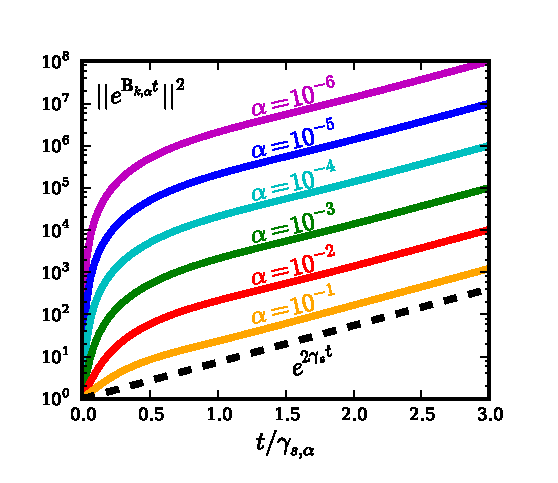
\includegraphics[width=0.45\textwidth]{max_en_growth}}
\caption{$G_{k,\alpha,\rm{max}}(t) = ||e^{\mathbf{B}_{k,\alpha} t}||^2$ for $k_x=0, k_y=1, \kappa=1$ for different values of the 2D adiabaticity parameter 
$\alpha$ compared to the energy growth $e^{2 \gamma_{s,\alpha,k} t}$ of the least stable eigenmode of  $\mathbf{B}_{k,\alpha}$. 
The time axis is normalized to $\gamma_{s,\alpha}$, which is different for each of the curves. This normalization makes the $e^{2 \gamma_{s,\alpha,k} t}$ line the same for all $\alpha$. 
$||e^{\mathbf{B}_{k,\alpha} t}||^2$ displays large non-exponential growth at early times that increases with decreasing $\alpha$.}
\label{max_en_growth}
\end{figure}

Non-normality manifests itself in its eigenvectors -- non-normal matrices or operators have non-orthogonal linear eigenvectors. For the HW model, each Fourier matrix $\mathbf{B}_k$ has two eigenvectors associated
with it. They are complex and take the form:

\beq
\label{lin_eigen_form}
\psi_{k,q} = \left( \begin{array}{cc} n_k \\ k_\perp \phi_k \end{array} \right)_q {\rm sin} \left( k_x x \right) e^{i k_y y + i k_z z} 
\eeq
where the subscript $q$ takes the values of $1$ and $2$, representing the two eigenvectors for each $k$. The two eigenvectors are different in that they have a different complex ratio $n_k/\phi_k$.
The two eigenvalues have different growth rates (the real part), but the same frequency, though with opposite sign.
As $\alpha \to 0$, the two eigenvectors become less orthogonal -- more parallel or anti-parallel to one another. When the eigenvectors are nearly anti-parallel and initialized with finite amplitude,
their superposition, which constitutes the total system at $k$, may linearly evolve so that the norm of the superposition grows faster than either individual eigenvector. A paradigmatic illustration
of this may be seen in a review by Schmid~\cite{schmid2007}.

\section{The Effect of Non-Normality on Turbulence}
\label{sec_non_norm_turb}

Linear non-normality is important for the effect it has on turbulence. It is most significantly a necessary condition for turbulence in subcritical systems that have only conservative nonlinearities 
(e.g. advective nonlinearities). However, non-normality can also impact non-subcritical systems, which have unstable linear eigenmodes like the HW system. 
Since certain superpositions of the linear eigenmodes can inject energy faster than the most unstable linear
eigenmode, there is the possibility that the energy injection into the turbulence is faster and at different wavenumbers than is suggested by linear eigenmode analysis. 

To illustrate this in the nonlinear HW model, we compare the fastest growing linear eigenmode growth rate $\gamma_{s,k}$ to the turbulent growth rate $\gamma_{t,k}$. 
In order to define the turbulent growth rate in general and specifically for the HW model, we employ a Fourier-decomposed energy dynamics analysis~\cite{camargo1995,friedman2012b,friedman2013}. 
Specifically, we take Eqs.~\ref{n_eq} and~\ref{phi_eq} and substitute the following:

\beqar
\label{subs_fourier}
n = \sum_{k} n_k \ {\rm sin} \left( k_x x \right) e^{i k_y y + i k_z z} \\
\phi = \sum_{k} \phi_k \ {\rm sin} \left( k_x x \right) e^{i k_y y + i k_z z},
\eeqar
where, again, $k$ stands for $(k_x,k_y,k_z)$.
Then, we multiply the resulting first equation by $n^*_{k'} \ {\rm sin} \left( k'_x x \right) e^{-i k'_y y - i k'_z z}$ and the second equation by 
$-\phi^*_{k'} \ {\rm sin} \left( k'_x x \right) e^{-i k'_y y - i k'_z z}$, take the volume integral and add the two equations together. The result is

\beqar
\label{Explicit_En_eqn}
\frac{1}{2} \diff{}{t} \left( |n_k|^2 + k^2_\perp |\phi_k|^2 \right) = -i k_y \kappa \phi_k n^*_k - \xi k_z^2 |n_k - \phi_k|^2 \nonumber \\
- D k^4_\perp \left( |n_k|^2 + k^2_\perp |\phi_k|^2 \right) + \sum_{k'} T(k,k'), \quad \quad
\eeqar
where, again, the energy $E_k$ is $\frac{1}{2} \left( |n_k|^2 + k^2_\perp |\phi_k|^2 \right)$, 
and the term $\sum_{k'} T(k,k')$ represents the nonlinear contribution (three-wave transfers between different $k$'s), 
which we do not write explicitly. This energy evolution equation may be written symbolically as

\beq
\label{dEdt_def}
\diff{E_k}{t} = \diff{E_{l,k}}{t} + \diff{E_{nl,k}}{t}
\eeq
where $\diff{E_{l,k}}{t}$ represents the terms that come from the linear terms in Eqs.~\ref{n_eq} and~\ref{phi_eq}, which are quadratic in the fluctuating
quantities $n_k$ and $\phi_k$ in Eq.~\ref{Explicit_En_eqn}. 
$\diff{E_{l,k}}{t}$ represents the injection of energy into the fluctuations from the free energy in the equilibrium gradients plus the dissipation from collisions and hyperdiffusion.
$\diff{E_{nl,k}}{t}$ represents $\sum_{k'} T(k,k')$ in  Eq.~\ref{Explicit_En_eqn} and comes from the nonlinear terms in Eqs.~\ref{n_eq} and~\ref{phi_eq}. 
The terms in $T(k,k')$ are triadic in the fluctuating quantities and account for the energy exchange between fluctuations with different $k$'s. 
They are also conservative when summed over all wavenumbers: $\sum_{k} \diff{E_{nl,k}}{t} = \sum_{k,k'} T(k,k') = 0$~\cite{camargo1995}.

Now, in quasi-steady state turbulence, the rate of net energy injection (or dissipation) into the fluctuations at each $k$ by the linear terms must be balanced by
the rate of energy removal (or deposition) from the nonlinear terms. This may be represented formally using growth rates:

\beqar
\label{steady_state}
\gamma_k \equiv  \displaystyle\lim_{T \to \infty} \frac{1}{T} \int_0^T \frac{dE_k/dt}{2 E_k} dt \nonumber \\
= \displaystyle\lim_{T \to \infty} \frac{{\rm{Log}}\left[ E_k(T)/E_k(0) \right]}{2 T} = 0.
\eeqar
The limit of the last expression vanishes -- as indicated -- for steady or quasi-steady state turbulence only.
From, Eqs.~\ref{dEdt_def} and~\ref{steady_state}, it follows that $ \gamma_k = \gamma_{l,k} + \gamma_{nl,k} = 0$.

We now associate the turbulent growth rate $\gamma_{t,k}$ discussed above with the linear rate of energy injection into the fluctuations $\gamma_{l,k}$ because $\gamma_{l.k}$
determines how fast and where in wavenumber space energy is injected into the turbulence.
$\gamma_{l,k}$, in other words, is the turbulence equivalent to the linear eigenmode growth rate $\gamma_{s,k}$~\cite{friedman2012b,terry2006b}. 
That is, in a linear simulation run for a sufficiently long time where transients die away, the calculation of $\gamma_{l,k}$ gives exactly $\gamma_{s,k}$.
Moreover, $\gamma_{l,k}$ is calculated from the spatial structures of the plasma state variables, so it is always well-defined, even in a turbulent plasma.

A turbulent system, which can be decomposed into a linear eigenvector basis, has $\gamma_{t,k} \le \gamma_{s,k}$ if the system is normal. Recall that in normal systems, the maximal
energy growth is given by the most unstable linear eigenmode. In other words, maximal growth is achieved when only the most unstable eigenmode has finite amplitude.
On the other hand, non-normal systems may grow faster when the more stable eigenmodes have finite amplitude than when they have none (see Fig.~\ref{max_en_growth}). 
It is therefore possible for $\gamma_{t,k} > \gamma_{s,k}$ in non-normal systems. 

\begin{figure}
\centerline{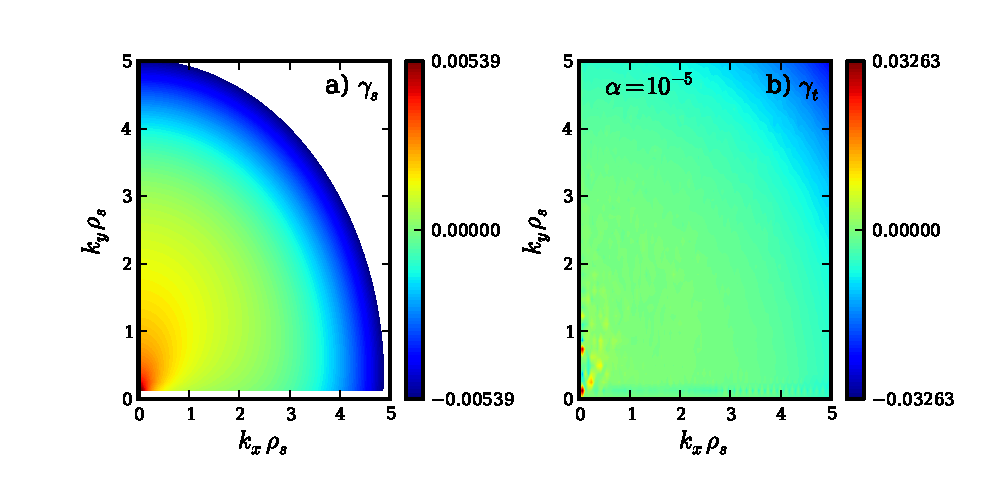
\includegraphics[width=0.52\textwidth]{alpha1e-5_gamma_s_t}}
\caption{{\bf a)} The eigenmode growth rate spectrum $\gamma_{s,k}$ and {\bf b)} the turbulent growth rate spectrum $\gamma_{t,k}$ for $\alpha = 10^{-5}, \kappa=1$. Note the different scales.}
\label{alpha1e-5_gamma_s_t}
\end{figure}

\begin{figure}
\centerline{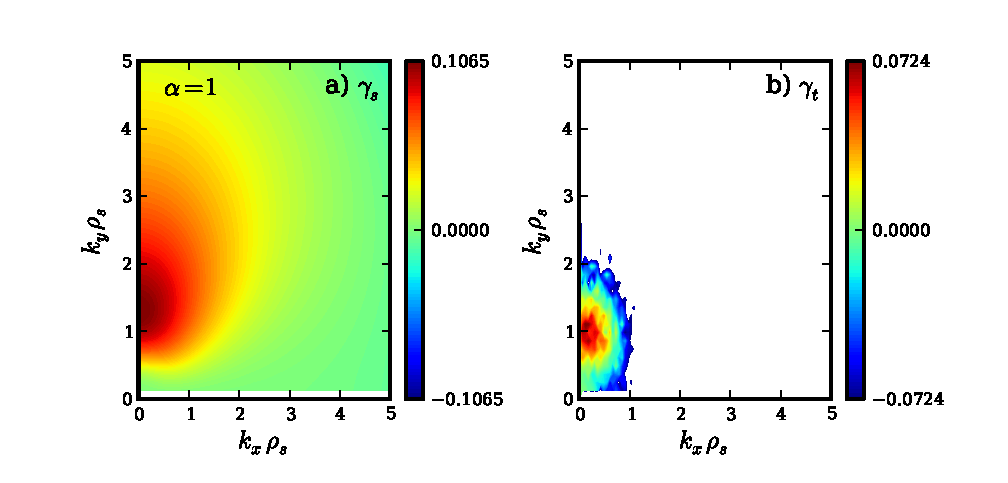
\includegraphics[width=0.52\textwidth]{alpha1_gamma_s_t}}
\caption{{\bf a)} The eigenmode growth rate spectrum $\gamma_{s,k}$ and {\bf b)} the turbulent growth rate spectrum $\gamma_{t,k}$ for $\alpha = 1, \kappa=1$.}
\label{alpha1_gamma_s_t}
\end{figure}

For the 2D HW model, we show
$\gamma_{s,k}$ and $\gamma_{t,k}$ for two different values of $\alpha$. In Fig.~\ref{alpha1e-5_gamma_s_t}, we show these growth rate spectra for $\alpha = 10^{-5}$, for which the system is
highly non-normal, and in Fig.~\ref{alpha1_gamma_s_t} for $\alpha = 1$, for which the system is very close to being normal. All calculations in this section use $\kappa=1$. 
Note the different scales used in all of the figures. In the highly
non-normal case, the turbulent growth rate is somewhat higher than the eigenmode growth rate for most values of $k_x,k_y$, and about 6 times higher where the spectrum peaks. For the more normal
case, in contrast, $\gamma_{t,k}$ is generally lower than $\gamma_{s,k}$, with the peak at nearly a factor of 2 less, with the peaks being at slightly different values of $k_y$.

\begin{figure}
\centerline{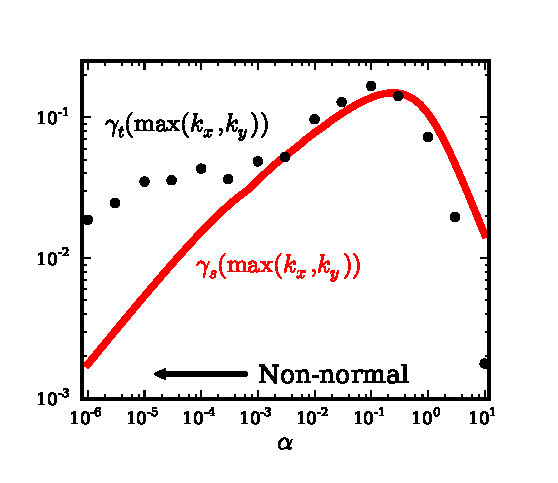
\includegraphics[width=0.4\textwidth]{gamma_max_vs_alpha}}
\caption{The eigenmode $\gamma_{s}$ and turbulent $\gamma_{t}$ growth rates as a function of $\alpha$, which controls the normality of the linear operator. All growth rates are peaks in $k_x-k_y$ space.}
\label{gamma_max_vs_alpha}
\end{figure}

We show the peak values for $\gamma_{s,k}$ and $\gamma_{t,k}$ in Fig.~\ref{gamma_max_vs_alpha} as a function of $\alpha$. The peak values always occur in $k$-space
at the lowest $k_x$ available to our system, corresponding to half of a period of a sine wave. The value of $k_y$ that gives the highest growth rate migrates upward as $\alpha$ increases,
as is clear from Figs.~\ref{alpha1e-5_gamma_s_t} and~\ref{alpha1_gamma_s_t}. Furthermore, as expected, when $\alpha$ is small ($\lesssim 10^{-3}$), $\gamma_{t,k} > \gamma_{s,k}$, with
$\gamma_{t,k} \gg \gamma_{s,k}$ as $\alpha \to 0$. Additionally, when $\alpha$ becomes larger and the system becomes more normal ($\gtrsim 10^{-1}$), $\gamma_{t,k} < \gamma_{s,k}$.

For both the normal and highly non-normal limits of the 2D HW model, $\gamma_{s,k}$ does a poor job of predicting $\gamma_{t,k}$ because $\gamma_{s,k}$ neglects the stable branch of the
dispersion relation -- the damped eigenmode. The importance of the stable eigenmode branch (or branches) 
has started to gain acceptance in the plasma community~\cite{baver2002}, although it has generally been used in normal
or nearly normal systems to explain turbulent saturation~\cite{terry2006b,hatch2011,makwana2011} ($\gamma_{t,k} < \gamma_{s,k}$). 
The case of highly non-normal turbulence and the associated increased turbulent excitation hasn't been understood as well. 
In fact, simulation and analysis of the 3D HW model (and extended models) is an area in which others have seen the effects of strong non-normal transient growth
but have not realized them as such~\cite{biskamp1995,drake1995,scott2002,scott2005,umansky2009,friedman2012b}.

\begin{figure}
\centerline{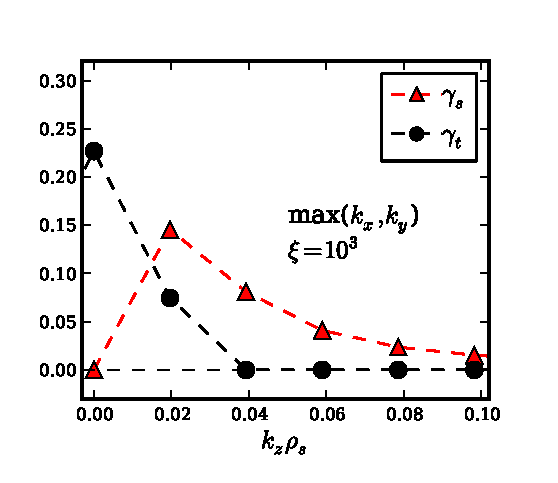
\includegraphics[width=0.4\textwidth]{gamma_max_vs_kz}}
\caption{The growth rates of the fastest growing eigenmode $\gamma_{s,k}$ and the of the turbulence $\gamma_{t,k}$ as a function of $k_z$ for the 3D HW model at $\xi = 10^3$. The most remarkable feature is
that the turbulent growth rate peaks at $k_z=0$ despite the stability of all linear eigenmodes at $k_z=0$.}
\label{gamma_max_vs_kz}
\end{figure}

As Biaskamp and Zeiler~\cite{biskamp1995} discovered, the 3D HW model nonlinear simulation has a fascinating property -- 
the turbulent energy injection is positive at $k_z = 0$ despite the fact that there can be no unstable linear eigenmodes at $k_z=0$.
In fact, for high enough values of $\xi$ ($\xi \ge 10^2$), more energy is injected at $k_z = 0$ than at finite $k_z$ (see Fig.~\ref{gamma_max_vs_xi} below for more details).
We show this in Fig.~\ref{gamma_max_vs_kz} using the eigenmode $\gamma_{s,k}$ and turbulent $\gamma_{t,k}$ growth rates, plotting them as a function of $k_z$.
The long-stated cause of this $k_z=0$ energy injection is a nonlinear instability~\cite{biskamp1995,drake1995}. 
The nonlinear instability works as follows: magnetic-field-aligned ($k_z=0$) convective cells transport density across the equilibrium density gradient, setting up $k_z=0$ density structures. 
These structures are unstable to drift waves, which grow as a secondary instability.
The secondary drift waves, which have finite $k_z$, nonlinearly couple to one another and reinforce the original convective cells (or generate new ones), leading to self-sustainment.

Although the instability is a nonlinear instability, the first part of the mechanism -- the transport of background density by the convective cells -- is a linear one. This process occurs at $k_z=0$
for which the adiabaticity parameter iz zero ($\alpha = k_z^2 \xi = 0$) meaning the linear matrix operator is highly non-normal and subject to transient growth.
So non-normal effects play a role in the 3D HW system for all $\xi$ due to the presence of $k_z=0$ structures.

\section{Non-Modal Linear Procedure To Calculate Turbulent Growth Rate}
\label{sec_nm_procedure}

In this section, we outline a procedure that uses quick and simple methods to approximate the turbulent growth rates $\gamma_{t,k}$.
We contend that the key to doing this is to successfully model the effect that the nonlinearities have on the linear (transient and possibly modal) processes.
First, we note that the advective nonlinearity terms in Eqs.~\ref{n_eq} and~\ref{phi_eq} have a common form -- a state variable multiplied by an inverse time scale:
$\tau_{nl}^{-1} \sim v_E k_\perp$.
This nonlinear time scale is generally associated with the eddy turnover or decorrelation time. We thus present a heuristic model of the nonlinearities 
as a randomizing force that acts on this characteristic nonlinear time scale. More specifically, this model is one in which 1) the turbulence begins as a random state, 
2) evolves linearly for a time $\tau_{nl}$, and 3) randomizes by nonlinear energy transfer, at which point the steps repeat.

We can calculate an effective growth rate from this model by starting with an ensemble of random initial conditions, evolving them linearly for a time $\tau_{nl}$, and
then taking the time and ensemble averaged growth rate of these curves.
In practice, this procedure can be greatly sped up and simplified. To see this, recall that the time evolution of the energy from an initial condition is

\beq
\label{E_t_from_u0}
E_k(t) = ||e^{\mathbf{B}_k t} u(0)||^2 = e^{\mathbf{B}_k t} u(0) u^{\dagger}(0) e^{\mathbf{B}_k^{\dagger}t}.
\eeq
Since we want the ensemble of initial conditions ($u(0)$'s) to be random normalized vectors with uncorrelated components, it follows that~\cite{camargo1998}

\beq
\label{E_t_ensemble_avg}
\left< E_k(t) \right>_{{\rm{ens}}} = \frac{1}{2} {\rm{tr}} \{ e^{\mathbf{B}_k t} e^{\mathbf{B}_k^{\dagger}t} \},
\eeq
where the normalization is $||u(0)||^2 = 1$. Mathematically, we define the non-modal growth rate $\gamma_{{\rm{nm}},k}$ as the time averaged instantaneous growth rate:

\beq
\label{gamma_nm_calc}
\gamma_{{\rm{nm}},k} = \frac{1}{\tau_{nl,k}} \int_0^{\tau_{nl,k}} \frac{\pdiff{E_k(t)}{t}}{2 E_k(t)} dt = \frac{1}{2 \tau_{nl,k}} \ {\rm{Log}} \left[ \frac{E_k(\tau_{nl,k})}{E_k(0)}\right].
\eeq
Taking $E_k(t)$ as the ensemble averaged energy calculated from Eq.~\ref{E_t_ensemble_avg} and setting $E_k(0) = 1$ for normalization, we find,

\beq
\label{gamma_nm}
\gamma_{{\rm{nm}},k} = \frac{1}{2 \tau_{nl,k}} \ {\rm{Log}} \left<  E_k(\tau_{nl,k}) \right>_{\rm{ens}}.
\eeq

Now, in order to obtain a simple and quick prediction of $\gamma_{{\rm{nm}},k}$, we must estimate $\tau_{nl,k}$ without having to calculate it directly from a turbulent simulation. 
We thus invoke the conjecture of \emph{critical balance}, which posits that the nonlinear time scale equals a characteristic linear time scale at all spatial scales~\cite{schekochihin2012}. 
This is a fair assumption in light of our discussion above, in which we showed that $\gamma_{l,k} = - \gamma_{nl,k}$.

There are a several possible linear time scales in the HW problem to use for $\tau_{nl,k}$ 
including the inverse linear eigenmode frequency and growth rates as well as certain times associated with transient growth curves. 
After trying a few of these different time scales, we have concluded that the one that works best is the inverse of the linear eigenmode frequency $\omega_{s,k}$
-- the imaginary part of the eigenvalues of the linear matrix operator $\mathbf{B}_k$.
Recall that the imaginary part of the linear eigenvalues is the same for both eigenvalues of $\mathbf{B}_k$, so there is no question of which to use. Because of this, unlike the eigenmode growth rates,
the frequency is robust no matter how nonorthogonal the eigenvectors. We thus arrive at our final definition for the non-modal growth rate:

\beq
\label{gamma_omega_def}
\gamma_{\rm{nm},k} = \frac{\omega_{s,k}}{4} \ {\rm{Log}} \left[ {\rm{tr}} \{ e^{\mathbf{B}_k \omega_{s,k}^{-1}} e^{\mathbf{B}^{\dagger} \omega_{s,k}^{-1}} \} \right].
\eeq
Note that the factor of $\frac{1}{4}$ is particular to two-field systems. Namely, the factor of $\frac{1}{2}$ coming from Eq.~\ref{E_t_ensemble_avg} is a consequence of the $2 \times 2$ dimensionality
of $\mathbf{B}_k$.

%The second linear time scale that we may use is the inverse of the linear growth rate. However, the eigenvalues of $\mathbf{B}_k$ have different growth rates (real parts). 
%Furthermore, we have argued that the eigenmode growth rates have little bearing on turbulence, especially for highly non-normal turbulence, 
%so it would be innappropriate to use either of the linear eigenmode growth rates as a proxy for the nonlinear time scale.
%Rather, we use the result itself, $\gamma_{{\rm{nm}},k}$, as the inverse of $\tau_{nl,k}$. Substituting $1/|\gamma_{{\rm{nm}},k}|$ for $\tau_{nl,k}$ in Eq.~\ref{gamma_nm_calc}, we get
%a transcendental equation:
%
%\beq
%\label{trans_gamma_nm}
%\gamma_{{\rm{nm}},k} = \frac{|\gamma_{{\rm{nm}},k}|}{2} \ {\rm{Log}} \left< E_k(1/|\gamma_{{\rm{nm}},k}|) \right>_{\rm{ens}}.
%\eeq
%We label this second non-modal growth rate $\gamma_{\gamma,k}$, and ultimately simplify this equation to
%
%\begin{figure}
%\centerline{\includegraphics[width=0.52\textwidth]{alpha1e-5_gamma_spec_compare}}
%\caption{a) The eigenmode growth rate spectrum $\gamma_{s,k}$,  b) the turbulent growth rate spectrum $\gamma_{t,k}$, c) the non-modal growth rate spectrum $\gamma_{\omega,k}$ d) and the 
%non-modal growth rate spectrum $\gamma_{\gamma,k}$ for the 2D HW model with $\alpha = 10^{-5}, \kappa=1$. Note the different scales.}
%\label{alpha1e-5_gamma_spec_compare}
%\end{figure}
%
%\begin{figure}
%\centerline{\includegraphics[width=0.52\textwidth]{alpha1_gamma_spec_compare}}
%\caption{a) The eigenmode growth rate spectrum $\gamma_{s,k}$,  b) the turbulent growth rate spectrum $\gamma_{t,k}$, c) the non-modal growth rate spectrum $\gamma_{\omega,k}$ d) and the 
%non-modal growth rate spectrum $\gamma_{\gamma,k}$ for the 2D HW model with $\alpha = 1, \kappa=1$.}
%\label{alpha1_gamma_spec_compare}
%\end{figure}
%
%
%\beq
%\label{gamma_pm2}
%\left< E_k(1/|\gamma_{\gamma,k}|) \right>_{\rm{ens}} = e^{\pm 2},
%\eeq
%where if $\left< E_k(t) \right>_{\rm{ens}}$ first reaches $e^2$, $\gamma_{\gamma,k}$ is positive, and if it first reaches $e^{-2}$, $\gamma_{\gamma,k}$ is negative.
%Therefore, finding $\gamma_{\gamma,k}$ amounts to a root-finding problem, which is not trivial, but is much simpler than a nonlinear simulation. 
%
%We test both of these non-modal growth rates to see if either or both produce good approximations of $\gamma_{t,k}$, especially in comparison to $\gamma_{s,k}$. 
%In Fig.~\ref{alpha1e-5_gamma_spec_compare}, we show the $\gamma_{\omega,k}$ and $\gamma_{\gamma,k}$ spectra for the 2D HW
%model for $\alpha=10^{-5}$ along with the eigenmode and turbulent spectra ($\gamma_{s,k}$ and $\gamma_{t,k}$), which we already provided in Fig.~\ref{alpha1e-5_gamma_s_t}. We do the same for
%$\alpha=1$ in Fig.~\ref{alpha1_gamma_spec_compare}. For the highly non-normal case ($\alpha = 10^{-5}$), $\gamma_{\omega,k}$ reproduces $\gamma_{t,k}$ in both magnitude and spectral shape. 
%$\gamma_{\gamma,k}$ is not close in any respect to $\gamma_{t,k}$. On the other hand, for the nearly normal case ($\alpha=1$), $\gamma_{\omega,k}$ does not resemble $\gamma_{t,k}$. 
%$\gamma_{\gamma,k}$ actually is fairly similar to $\gamma_{s,k}$, but with a slightly decreased amplitude, making it a closer match to $\gamma_{t,k}$, though it is still not similar for all $k$.

\begin{figure}
\centerline{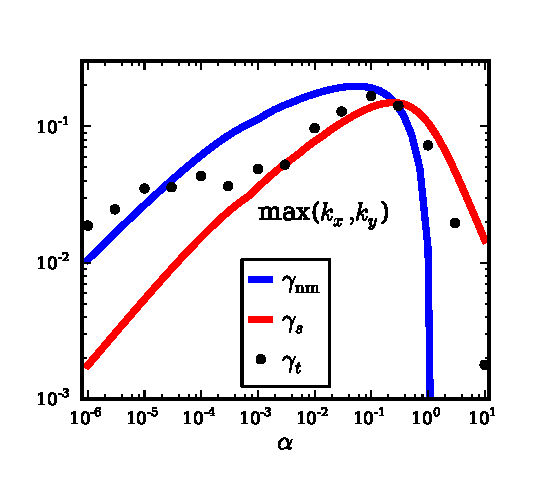
\includegraphics[width=0.45\textwidth]{gamma_max_with_nm}}
\caption{Comparison of the non-modal growth rate $\gamma_{\rm{nm},k}$ to the eigenmode $\gamma_{s}$ and turbulent $\gamma_{t}$ growth rates as a function of $\alpha$
for the 2D HW model. All growth rates are peaks in $k_x-k_y$ space.}
\label{gamma_max_with_nm}
\end{figure}

The peak non-modal growth rate prediction agrees fairly well with the turbulent growth rate for highly non-normal 2D HW turbulence as seen in Fig.~\ref{gamma_max_with_nm}. For $\alpha \le 10^{-4}$,
in which the system is fairly non-normal, $\gamma_{\rm{nm},k}$ predicts $\gamma_{t,k}$ quite accurately, especially compared to the eigenmode prediction. 
As the system becomes more normal, $\gamma_{t,k}$ and $\gamma_{\rm{nm},k}$ diverge, with $\gamma_{t,k}$ taking on values between $\gamma_{s,k}$ and $\gamma_{\rm{nm},k}$, 
but generally closer to $\gamma_{s,k}$ for $\alpha \gg 10^{-3}$. 

This indicates that some assumption in our procedure doesn't work well for systems that are normal or nearly normal. Namely, our assumption
of complete randomization by the nonlinearities breaks down. The nonlinearities only partially randomize the turbulence in the weakly non-normal case such that
the turbulence at a given $k$ always consists primarily of the unstable eigenmode. The stable eigenmode never accounts for a significant portion of the energy in the turbulence.
Makwana et al.~\cite{makwana2011} developed a condition based on the ratio of the stable to unstable eigenmode growth rates that can be used to determine the significance of the stable eigenmode. 
They determined that for $\alpha \ge 10^{-1}$, the stable eigenmode receives very little energy, explaining why our procedure does not work well in the normal limit for the 2D HW model.

\begin{figure}
\centerline{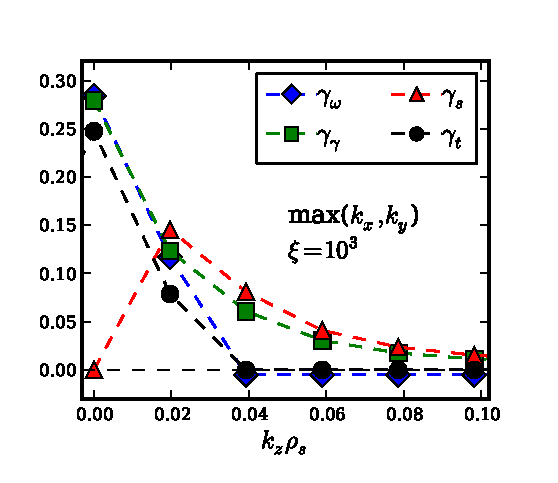
\includegraphics[width=0.4\textwidth]{gamma_max_vs_kz_with_nm}}
\caption{Comparison of the non-modal growth rate $\gamma_{\rm{nm},k}$ to the growth rates of the fastest growing eigenmode $\gamma_{s,k}$ 
and the of the turbulence $\gamma_{t,k}$ as a function of $k_z$ for the 3D HW model with $\xi = 10^3$. The non-modal growth rate correctly predicts the growth rate dominance of the $k_z=0$ mode
despite the $k_z=0$ eigenmode stability.}
\label{gamma_max_vs_kz_with_nm}
\end{figure}

We do the same comparison for the 3D HW model as we did for the 2D HW model. However, there is one additional subtelty when considering the 3D model. In the 3D model, for $k_z=0$, the linear
eigenmode frequency is zero ($\omega_{s,k_z=0} = 0$), so $\gamma_{\rm{nm},k_z=0}$ is not well defined (see Eq.~\ref{gamma_omega_def}). 
%We could, in fact, make the argument that since $\omega_{s,k_z=0} = 0$, or by critical balance $\tau_{nl,k_z=0} \to \infty$, it would be proper to equate $\gamma_{\rm{nm},k_z=0}$ with $\gamma_{s,k_z=0}$
%since all transients die away in the long time limit. 
Thus, we use $\omega_{s,k_z=0.02}$ -- where $k_z=0.02$ is the lowest finite value of $k_z$ available to our system -- in place of
$\omega_{s,k_z=0}$ in the calculation of $\gamma_{\rm{nm},k_z=0}$. We contend that the nonlinear instability, which most strongly couples $k_z=0$ and $k_z=0.02$ modes, has its time scale set
by the drift waves, not the convective cells, making $1/\omega_{s,k_z=0.02}$ a good proxy for $\tau_{nl,k_z=0}$. 

%One may recall that the drift waves are actually secondary, and therefore, they feed
%off of the $k_z=0$ density structures, so the appropriate scale length to use for $\omega_{s,k_z=0.02}$ is not given by $\kappa$, but by the scale length of the density structures. We don't deal
%with this complication and assume the scale length of the fluctuating density structures is the same as the background.

\begin{figure}
\centerline{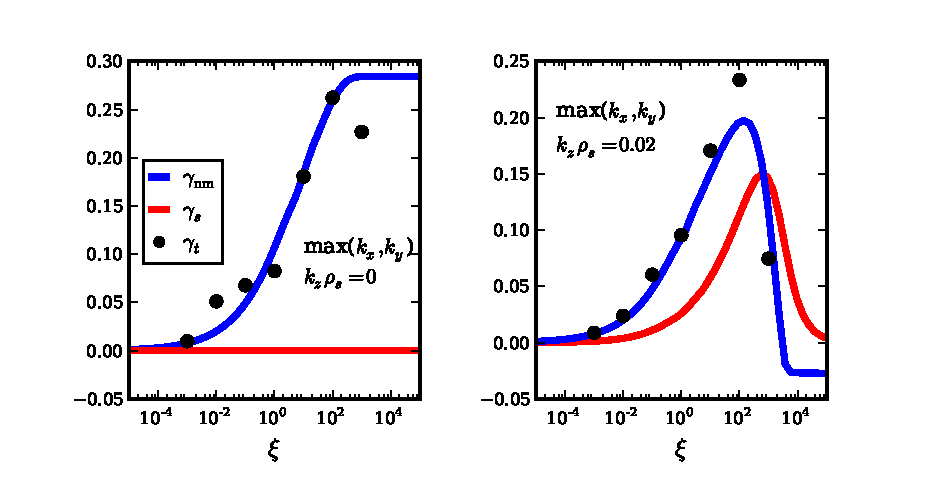
\includegraphics[width=0.52\textwidth]{gamma_max_vs_xi}}
\caption{Comparison of the peak non-modal growth rate $\gamma_{\rm{nm},k}$ to that of the fastest growing eigenmode $\gamma_{s,k}$ 
and the turbulence $\gamma_{t,k}$ as a function of $\xi$ for the 3D HW model at {\bf a)} $k_z \rho_s = 0$ and {\bf b)} $k_z \rho_s \approx 0.02$. }
\label{gamma_max_vs_xi}
\end{figure}

Despite these complications at $k_z=0$, our non-modal method of calculating $\gamma_{\rm{nm},k}$ approximates $\gamma_{t,k}$ remarkably well as seen in Figs.~\ref{gamma_max_vs_kz_with_nm}
and~\ref{gamma_max_vs_xi}. Most importantly, it correctly predicts that $\gamma_{t,k_z=0} > 0$. 
Therefore, non-modal calculations explain why the 3D HW model can be dominated by the nonlinear instability rather than a linear drift wave instability. 
Simply put, the transient growth rate is by far the largest at $k_z=0$ for $\xi \gg 10^2$, so the nonlinear instability is energetically favored over the primary drift wave instability.
For $\xi \le 10^2$, the $k_z=0$ nonlinear instability has comparable growth rate to the drift wave instability, so neither dominates.

\section{Prediction of Control Parameter for Subcritical Turbulent Onset}
\label{sec_subcrit_prediction}

In both hydrodynamic and plasma systems, it is important to be able to predict for a given set of parameters whether the system will be turbulent or not.
Put another way, it is useful to map out the point, line, or manifold in parameter space that divides turbulent and laminar solutions.
In many hydrodynamic systems with sheared flow, there is generally a single control parameter -- the Reynold's number $Re$~\cite{drazin1981}. For high enough $Re$ such systems
can be turbulent, but for low $Re$ they are always laminar.
Normal systems will undergo a bifurcation from a laminar to non-laminar state when the control parameters are such that at least one of the linear eigenmodes is unstable~\cite{grossmann2000}.
In general, this is not true for non-normal systems. In many non-normal systems, turbulence can be sustained when all linear eigenmodes are stable -- the case of subcritical turbulence. 

\begin{figure}
\centerline{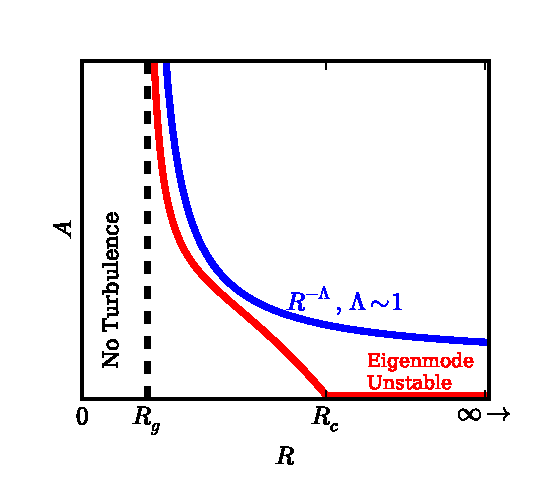
\includegraphics[width=0.4\textwidth]{subcritical_diagram}}
\caption{Diagram of a control parameter $R$ versus perturbation amplitude $A$ for two subcritical systems. The first curve (top blue one with $(R-R_g)^{-\lambda}$ label) represents a system with no
eigenmode instability for any $R$, but which is stable to finite amplitude perturbations for $R > R_g$. 
The second (bottom red one with label of ``Eigenmode Unstable'') represents a system with a linear eigenmode instability for $R \ge R_c$, and finite amplitude
instability for $R_g < R < R_c$.}
\label{subcritical_diagram}
\end{figure}

Subcritical systems fall into two categories: those that have stable eigenmodes for all values of the control parameter, and those that have unstable eigenmodes
when the control parameter becomes large (or small) enough. We illustrate these two categories with a diagram in Fig.~\ref{subcritical_diagram}. 
The upper curve represents the first kind of subcritical system in which no unstable eigenmodes exist for any value of the control parameter $R$. In this
case, there is some transitional value of $R$, labeled $R_g$, below which turbulence cannot occur. When a perturbation with amplitude above the line occurs in the system due to external input or noise, 
turbulence will be excited. Perturbations with amplitude below the line will decay away. Clearly, the higher the value of $R$, the smaller the perturbation needs to be to excite turbulence.
Experimental evidence and theoretical arguments show this curve should have a $(R-R_g)^{-\lambda}$ dependence, with $\lambda \sim 1$~\cite{grossmann2000}.
A paradigmatic example of this kind of system is Hagen-Poisuille pipe flow -- flow in a cylindrical pipe with a parabolic flow profile -- for which $R_g \approx 2000$.

The lower curve represents the second kind of subcritical system. Above a critical value of the control parameter $R_c$, the system is linearly unstable. But, for $R_g < R < R_c$, the system is
unstable to finite amplitude perturbations, or ``nonlinearly'' unstable. A paradigmatic example of this is Poissuille channel flow -- the rectangular analog of pipe flow -- for which
$R_c = 5772$ and $R_g \approx 1000$~\cite{grossmann2000}. Most subcritical magnetically-confined plasma systems fall into this category. It is perhaps easy to be fooled into believing that the turbulence
in such systems is due to eigenmode instability even though it may not be. 
In either case, one of the most important predictions is the minimum turbulent control parameter $R_g$, which is sometimes called the ``transitional'' value of the control parameter. Given that this problem is many decades old
and still unsolved, it is a tall order to predict $R_g$ without nonlinear simulations. We nevertheless make an attempt.

The HW model in an unsheared magnetic slab is not subcritical in either the 2D or 3D cases, as implied by Figs.~\ref{gamma_max_vs_alpha} and~\ref{gamma_max_vs_kz}. It is subcritical in a highly sheared
magnetic field~\cite{drake1995}, but the eigenmodes of the linear operator in that case are not sinusoidal, making our non-modal analysis more difficult. 
Biskamp et al.~\cite{biskamp1995}, however, artificially modified the
3D HW model to remove the linear drive by taking the $z$ average of the $\kappa \pdiff{\phi}{y}$ term in Eq.~\ref{n_eq}, effectively eliminating the $k_z \ne 0$ drive. This leaves only the $k_z = 0$
component of the drive term. Since the $k_z = 0$ eigenmodes are stable but $k_z = 0$ structures can access the free energy (positive $\gamma_t$ in Fig.~\ref{gamma_max_vs_kz}), this system is subject
to subcritical turbulence.

We show that the system is subcritical in Fig.~\ref{crit_amp_dependence}. In Fig.~\ref{crit_amp_dependence} a), we plot the energy versus time for fluctuations that are initialized with different amplitudes. 
The fluctuations initialized with high enough amplitude lead to turbulence. 
Otherwise, the fluctuations grow transiently, but do not reach high enough amplitude for the nonlinearities to bootstrap the process,
so they decay away (we set the diffusion and viscosity coefficient $D$ to $0.5$ in this section so that the decay occurs on a short enough time scale to keep the simulations short). 
This finite amplitude turbulence threashold, as described above, is a key indicator of subcritical turbulence.

In Fig.~\ref{crit_amp_dependence} b), we show the amplitude threashold curve -- like that of Fig.~\ref{subcritical_diagram} -- for the subcritical 3D HW model. We obtain the points from nonlinear simulations
and fit them to a function of the form $A = a (\kappa - \kappa_g)^{- \lambda}$, where $A$ is the lowest initial energy amplitude that leads to turbulence for each value of $\kappa$. The least-squares fitting provides optimal values
for the parameters $a, \kappa_g, \rm{and} \lambda$. As expected for shear flows, $\lambda \sim 1$.

\begin{figure}
\centerline{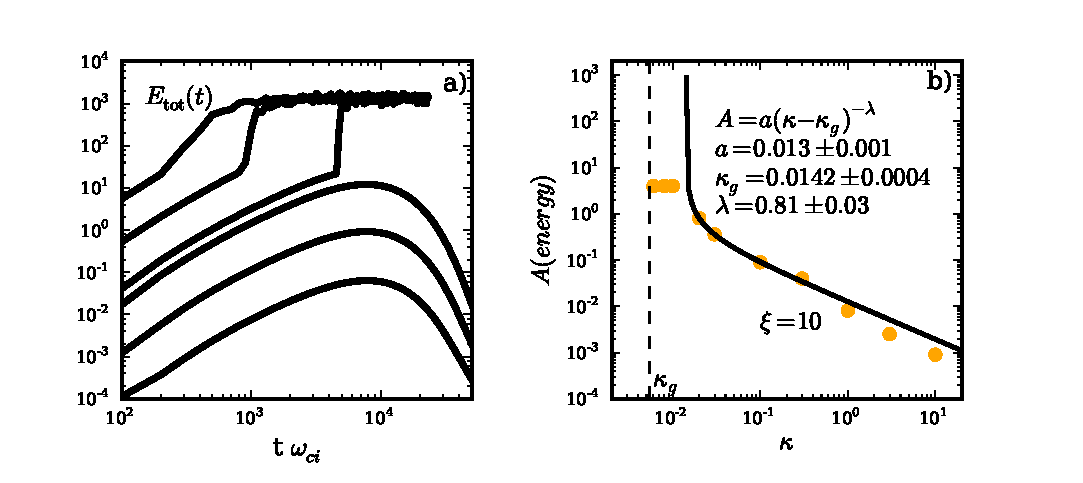
\includegraphics[width=0.52\textwidth]{crit_amp_dependence}}
\caption{{\bf a)} Total energy evolution of fluctuations of the modified 3D HW model with $\xi=10$ and $\kappa=1$ where the initial perturbations are set to different amplitudes. 
All initial perturbations are initialized randomly in the $y$ and $z$ directions and with a Guassian in the $x$ direction. 
There is a critical initial amplitude threashold above which turbulence develops and maintains itself and below which turbuelence never develops and the fluctuations decay away. 
{\bf b)} The amplitude threashold as a function of $\kappa$ for $\xi=10$. The points are obtained from nonlinear simulations like those in part a) with each point indicating the minimum amplitude needed for the simulation
to become turbulent. The line is a fit to the points with the functional form $a (\kappa-\kappa_g)^{- \lambda}$.}
\label{crit_amp_dependence}
\end{figure}

In this subcritical system, we predict the line in $\xi-\kappa$ parameter space that divides the space into an area that permits turbulent solutions and an area that does not. That is, we predict
$\kappa_g(\xi)$. We show the answer that we obtain from nonlinear simulations along with our non-modal prediction in Fig.~\ref{subcrit_param_space}. To obtain $\kappa_g(\xi)$ from the nonlinear simulations,
rather than mapping out curves like those in Fig.~\ref{crit_amp_dependence} b), we simply start all simulations with a large initial amplitude ($A = 10^4$) and vary $\kappa$ until we find the minimum $\kappa$ that
sustains turbulence (see Fig.~\ref{kappa_en_ev} for an example).

Our method
of prediction is to find the line in $\xi-\kappa$ space at which $\gamma_{\rm{nm}} = 0$, where $\gamma_{\rm{nm}}$ is maximized over $k_x$ and $k_y$. We plot this line in Fig.~\ref{subcrit_param_space}

\begin{figure}
\centerline{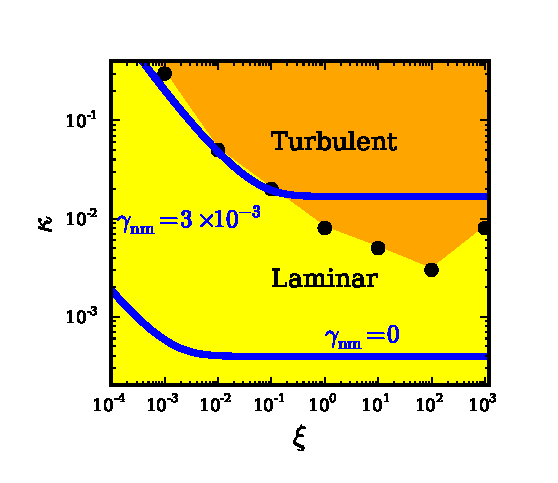
\includegraphics[width=0.4\textwidth]{subcrit_param_space}}
\caption{The non-modal curve $\gamma_{\rm{nm}}(\kappa,\xi) = 0$, which defines our prediction of the transitional value of $\kappa(\xi)$ for the subcritical 3D HW model. The points represent the
transitional values of $\kappa(\xi)$ based on full nonlinear simulations.}
\label{subcrit_param_space}
\end{figure}


\begin{figure}
\centerline{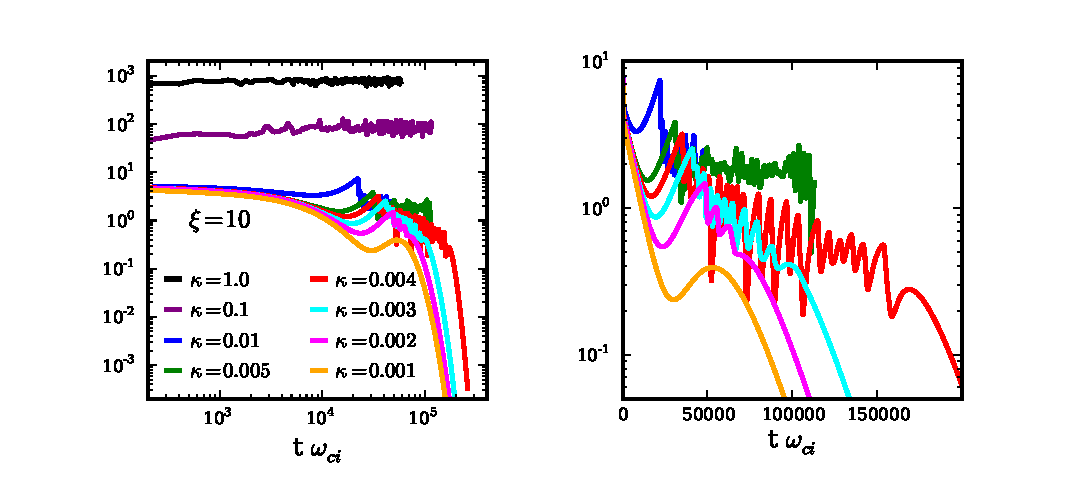
\includegraphics[width=0.52\textwidth]{kappa_en_ev}}
\caption{$E_{\rm{tot}}(t)$ from full nonlinear simulations of the subcritical 3D HW model. The curves that reach a quasi-steady-state value represent sustained subcritically turbulent states. 
Those that decay for large time have values of $\kappa$ too small to sustain turbulence. The transitional value $\kappa_g$ is the smallest value of $\kappa$ for which turbulence is sustained.}
\label{kappa_en_ev}
\end{figure}


\begin{acknowledgments}
This work was supported by the National Science Foundation (Grant PHY-1202007)
\end{acknowledgments}

%%%%%%%%%%%%%%%%%%%%%%%%%%%%%%%%%%%%%%%%%%%%%%%%%%%%%%%%%%%%%%%%%%%%%%%%%%%

%\bibliographystyle{phaip}
\bibliography{refs}

\end{document}
